\section{Method}

The program can be thought of a modifed image stitching pipline, with stages:
\begin{enumerate}
	\item Find Surf features in input images
	\item Estimate homographies between input images
	\item Create the virtual camera
	\item Pan/Tilt and Zoom with virtual camera to create transformantion-matrix
	\item Create a composite transformation matrix.
	\item Apply transformations on input images.
	\item Blend transformed images.
\end{enumerate}

In this particular implementation three images depicting a soccer game were used, as can be seen in fig. \ref{fig:input}. The most important functionality from OpenCV can be found in appendix \ref{appendix:opencv}.

\begin{figure*}[t]
	\centering
	\begin{subfigure}[t]{0.3\textwidth}
		\centering
		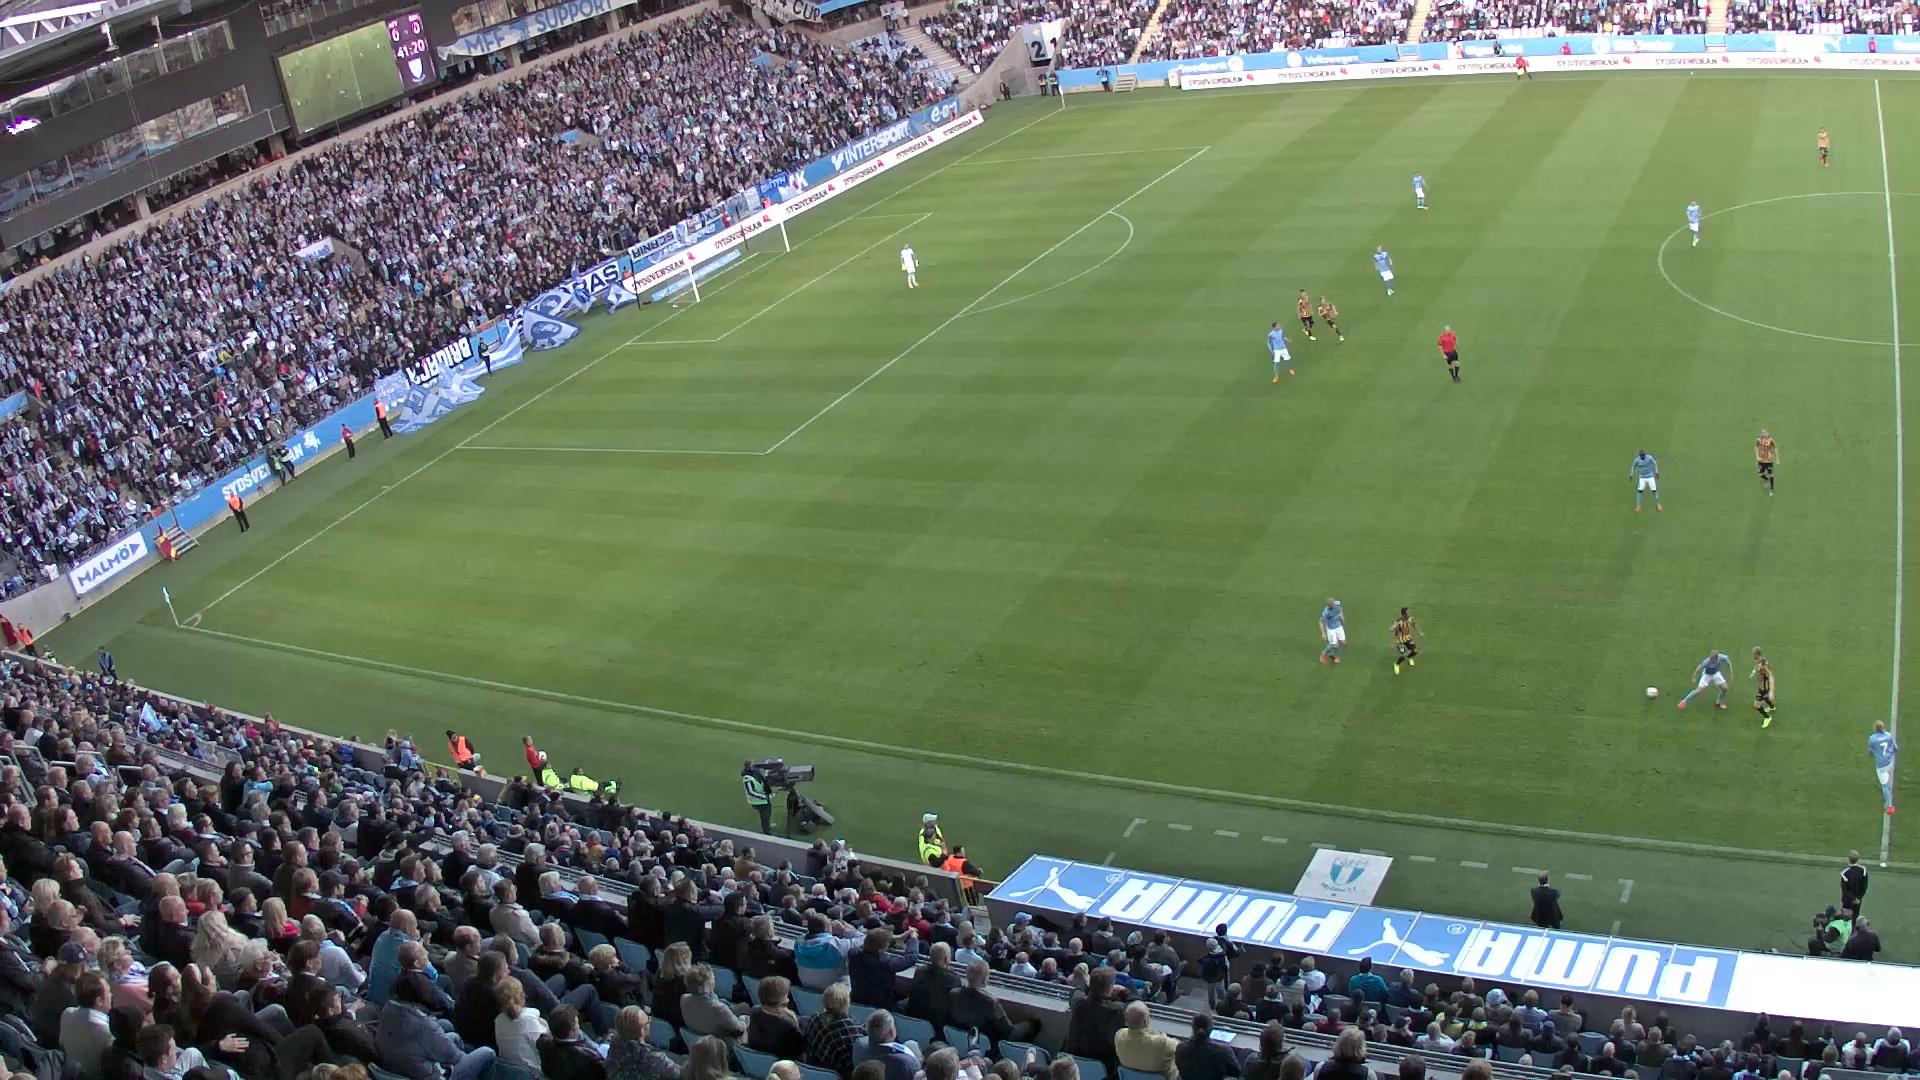
\includegraphics[width=\textwidth]{../data/20150521_194353_C1D8.jpg}
		\caption{1}
	\end{subfigure}
	\begin{subfigure}[t]{0.3\textwidth}
		\centering
		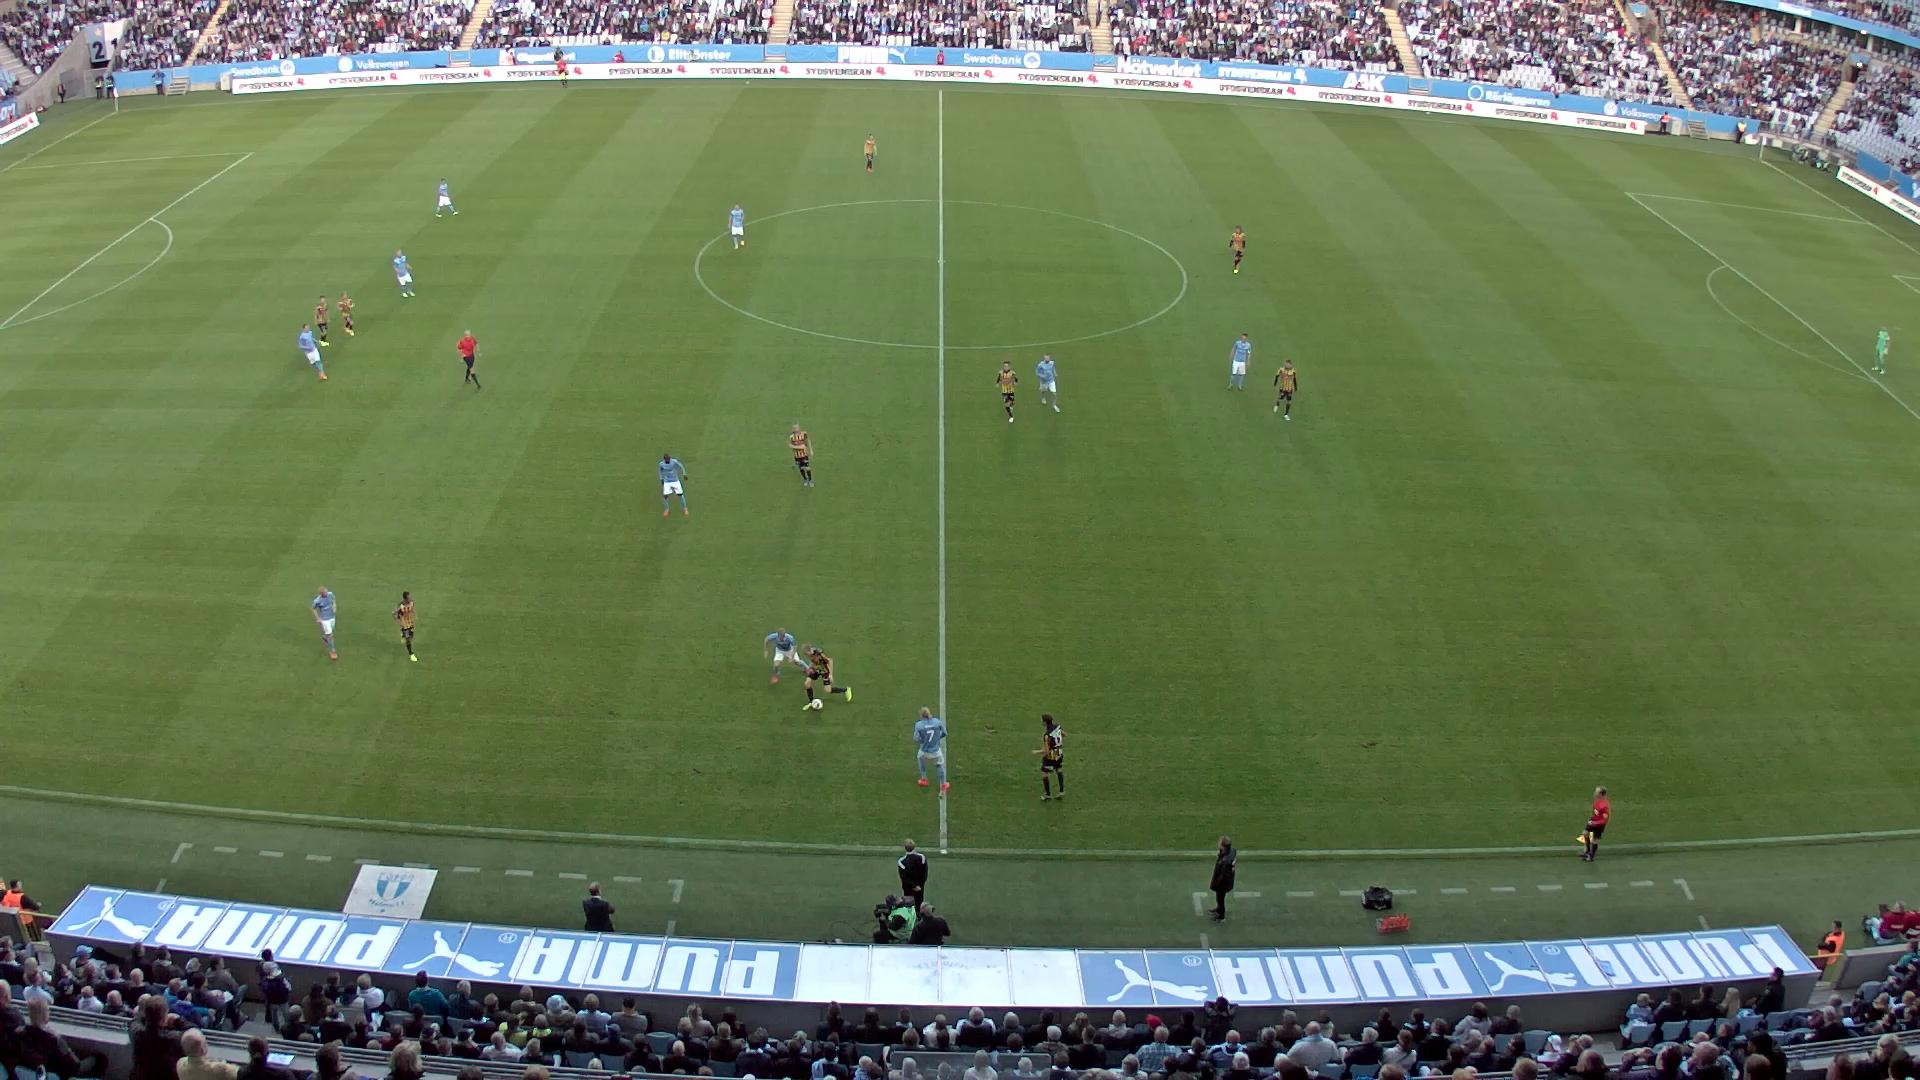
\includegraphics[width=\textwidth]{../data/20150521_194353_FD1E.jpg}
		\caption{2}
	\end{subfigure}
		\begin{subfigure}[t]{0.3\textwidth}
		\centering
		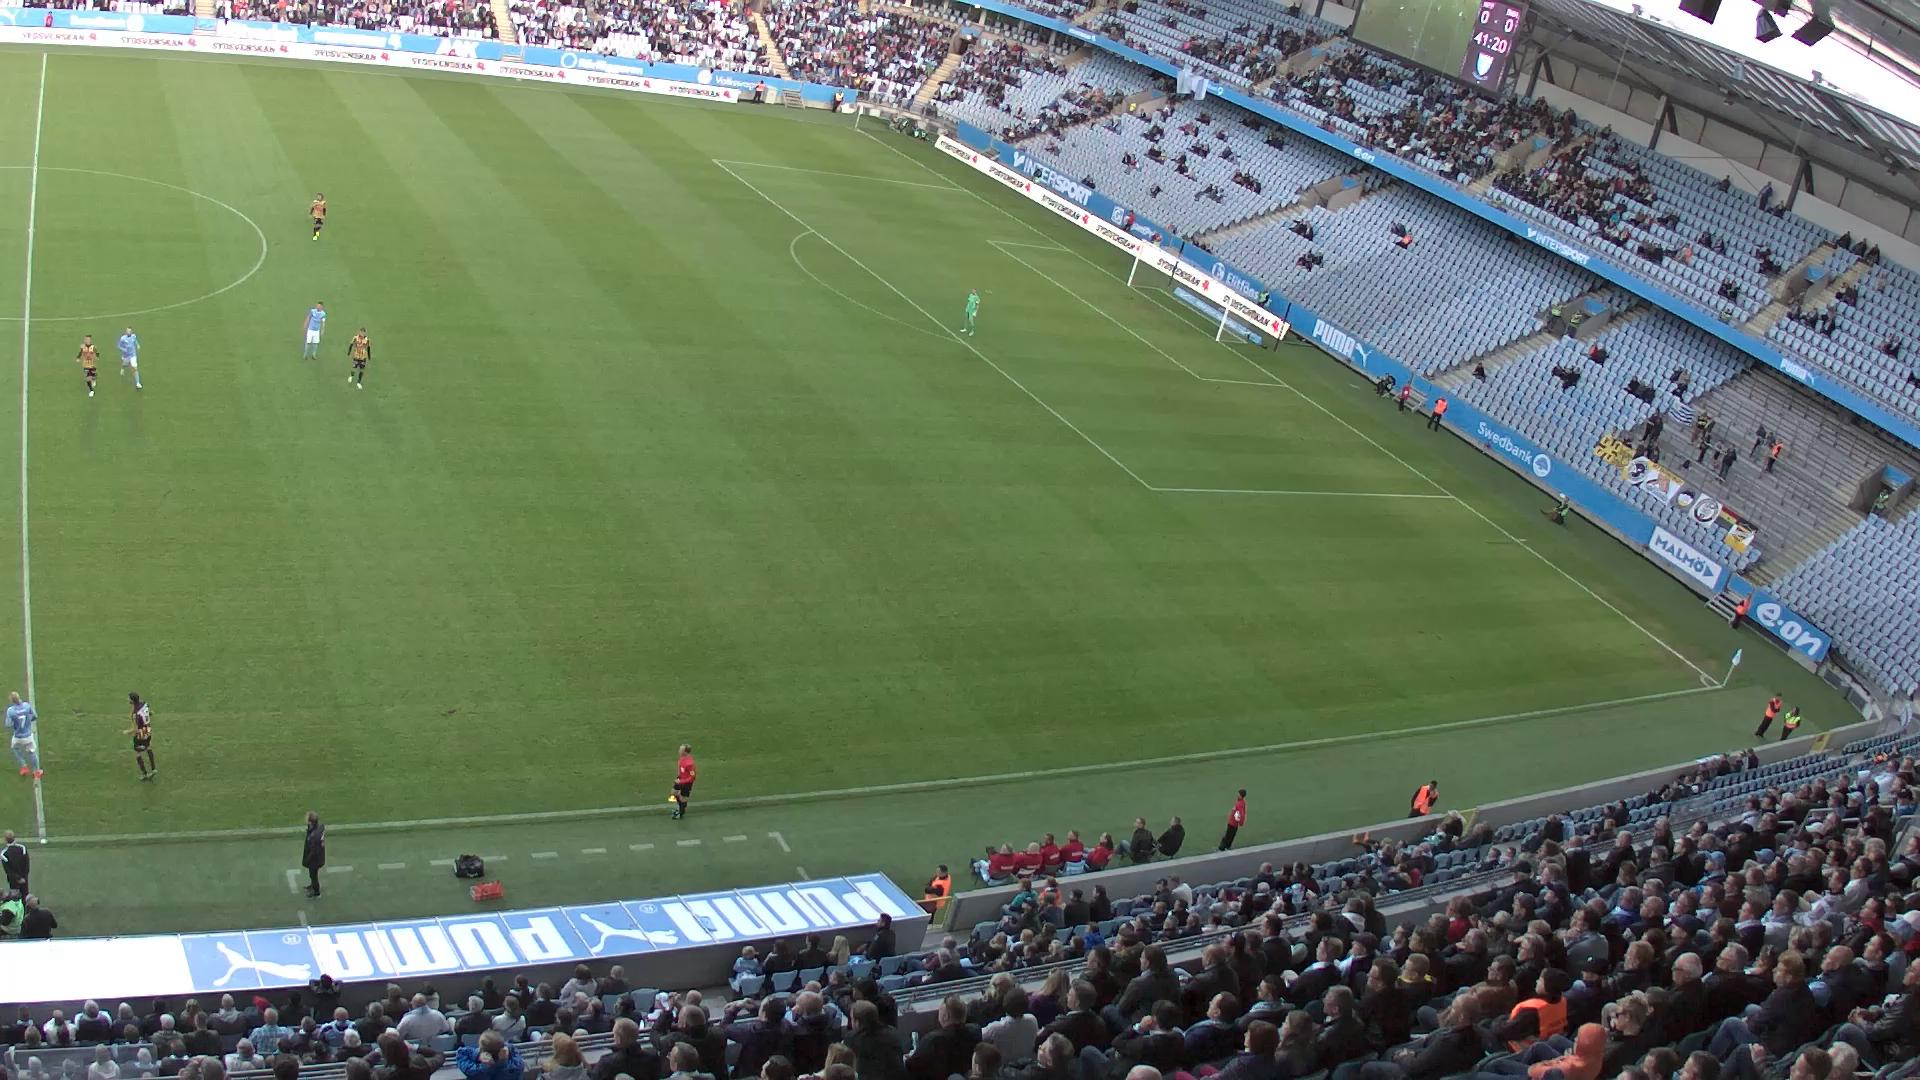
\includegraphics[width=\textwidth]{../data/20150521_194353_49E3.jpg}
		\caption{3}
	\end{subfigure}
	\caption{input images}
	\label{fig:input}
\end{figure*}

\subsection{Stitching}
This text only refers to stitching of two images, the same concept can be expanded for multiple images.

The stitching can be divided into two parts.
The first one is to find a relation, homography, between two images.
In other words where an image {\it fits} in the other image.
The other part is to combine or blend the images to make the transition between them as smooth as possible.

To find a relation between two images, mutual points have to be found.
This is done using a point detector which should find interest points in both images.
Then the points need a value for the possibility of matching points that are similar.
Here a feature descriptor is needed.
In this project a method called SURF has been used.
It includes both a detector and descriptor.
After SURFing the images the descriptors of the points are matched.
This matching is very likely to contain outliers, however, the RANSAC method can be used to avoid influence of the outliers when calculating the homography between the images.

The blending of the two images consists of three steps.
First the previously calculated homography is used to get the images in the same perspective.
Here there is an overlap between the images.
This overlap is weighted with a value $w_1$ for the left image and $w_2 = 1 - w_1$ for the right one.
In this project $w_1$ has been calculating using either a linear (equation \ref{eq:method:stitching:linear}) or sigmoid (equation \ref{eq:method:stitching:sigmoid}) function.
\begin{equation} \label{eq:method:stitching:linear}
  w_1 = -a x + b
\end{equation}
\begin{equation} \label{eq:method:stitching:sigmoid}
  w_1 = \frac{e^{-0.1(x - x_d)}}{1 + e^{-0.1(x - x_d)}}
\end{equation}
Here $a$, $b$ and $x_d$ are adapted to fit the overlap of the images.
With the start and end of the overlap in the x-direction a and b are set so that $w_1 = 1$ on the left end and $w_1 = 0$ on the other.
$x_d$ is just set to be the in the middle of the overlap in the x-direction.
At last the weighted images are stitched together.


\subsection{Virtual PTZ camera}
Using the decomposition in (\ref{eq:homodecomp}) we can transform the problem into three rotations, where we only really need to use two of them, the panning rotation around the camera Y-axis and rotation around the camera X-axis after the panning has been applied.
The rotational matrices are implemented as follows in (\ref{eq:pan}) and (\ref{eq:tilt})
	\begin{align}		
		R_{pan}&=\begin{pmatrix} 
			\cos(\theta_y) & 0 & -\sin(\theta_y) \\
			0 & 1 & 0 \\
			\sin(\theta_y) & 0 & \cos(\theta_y)
		\end{pmatrix} \label{eq:pan} \\
		R_{tilt} &=\begin{pmatrix}
			1 & 0 & 0 \\
			0 & \cos(\theta_x) & -\sin(\theta_x) \\
			0 & \sin(\theta_x) & \cos(\theta_x)
		\end{pmatrix} \label{eq:tilt}
	\end{align}
	For the particular input images in fig. \ref{fig:input}, the cameras were slighty tilted , with an estimated initial tilt angle of $\approx 0.47$ radians.\footnote{The exact estimated angle was 0.47179832679 radians.}
	This means that if we want our panning axis to coincide with the panning axis of the input images, we first need to apply a tilting of $-0.47$ radians, and then apply our panning matrix, (\ref{eq:pan}) and then our tilting matrix. 
	The ''initial tilt correction'' can be written in matrix form as (\ref{eq:tiltinit}).
	\begin{multline}
		R_{tiltCorr}=\begin{pmatrix}
			1 & 0 & 0 \\
			0 & \cos(-\theta_{tiltinit}) & -\sin(-\theta_{tiltinit}) \\
			0 & \sin(-\theta_{tiltinit}) & \cos(-\theta_{tiltinit})
		\end{pmatrix} = \\
		=\begin{pmatrix}
			1 & 0 & 0 \\
			0 & \cos(\theta_{tiltinit}) & \sin(\theta_{tiltinit}) \\
			0 & -\sin(\theta_{tiltinit}) & \cos(\theta_{tiltinit})
		\end{pmatrix}
		\label{eq:tiltinit}
	\end{multline}
	where $\theta_{tiltinit} \approx 0.47$ radians.

	The zoom is implemented as stated in (\ref{eq:zoom}).
	The matrices are finally multiplied together to a single composite matrix, $H_{perspective}$, see (\ref{eq:PTZcomp})

	\begin{equation}
		H_{perspective}=KZR_{tilt}R_{pan}R_{tiltCorr}K^{-1}
		\label{eq:PTZcomp}
	\end{equation}
	where K are the camera calibration matrices.
	As stated in the theory section, the homographies applied on the images are variants of a composite matrix defined as in (\ref{eq:comp}).

	\begin{equation}
		H_{composite}=H_{perspective}H_{stitching}
		\label{eq:comp}
	\end{equation}
	Where $H_{stitching}$ is the homography produced by the stitching algorithm, invidiual for each image. Note that the stitching transform is applied prior to the perspective transforms. % is it not the other way around

